\documentclass[a4paper, reqno]{amsart}

\usepackage{a4wide}

% Amsmath
\usepackage{amsmath}
\usepackage{amssymb}

% Algorithms
\usepackage{algorithm}
\usepackage{url}

\usepackage{pythonhighlight}

% Figures
\usepackage{graphicx}

% Pretty tables
\usepackage{booktabs}

% Color (temp)
\usepackage{color}

% Math operators
\DeclareMathOperator{\Div}{div}
\DeclareMathOperator{\Curl}{curl}
\DeclareMathOperator{\Grad}{grad}

% Vector spaces
\newcommand{\R}{\mathbb{R}}
\newcommand{\M}{\mathbb{M}}
\newcommand{\N}{\mathbb{N}}
\newcommand{\Poly}[1]{\mathcal{P}^{#1}}

% Measures
\newcommand{\dx}{\,\mathrm{d}x}
\newcommand{\ds}{\,\mathrm{d}s}
\newcommand{\dX}{\,\mathrm{d}X}

% Project names
\newcommand{\dolfin}{\textrm{DOLFIN}}
\newcommand{\fenics}{\textrm{FEniCS}}
\newcommand{\ufl}{\textrm{UFL}}
\newcommand{\ffc}{\textrm{FFC}}

% Misc
\newcommand{\triang}{\mathcal{T}}
\newcommand{\foralls}{\forall \,}
\newcommand{\assumption}[1]{A#1}
\newcommand{\inner}[2]{\langle #1, #2 \rangle}
\newcommand{\average}[1]{[#1]}
\newcommand{\ddt}[1]{\frac{\partial #1}{\partial t}}

% Theorem styles
\newtheorem{thm}{Theorem}[section]
\newtheorem{lem}[thm]{Lemma}
\newtheorem{cor}[thm]{Corollary}
\newtheorem{example}[thm]{Example}
\newtheorem{remark}{Remark}

% Equation numbering
\numberwithin{equation}{section}

% Sizes
\newcommand{\figurewidth}{0.9\textwidth}

%
\newcommand{\heart}{\Omega^H}
\newcommand{\torso}{\Omega^T}

%------------------------------------------------------------------------------
\title{Adjoint sensitivity analysis of a cardiac model to cellular
  conductivities: informal notes}

\author{Marie E. Rognes, Johan E. Hake, Molly M. C. Maleckar and
  Patrick E. Farrell}
%% \thanks{Center for Biomedical Computing at Simula Research Laboratory,
%%   P.O. Box 134, 1325 Lysaker, Norway (meg@simula.no). This work is
%%   supported by a Center of Excellence grant from the Research Council
%%   of Norway to the Center for Biomedical Computing at Simula Research
%%   Laboratory.}
\pagestyle{myheadings}
\thispagestyle{plain}
%\markboth{MARIE E. ROGNES}{Adjoining a cardiac model}

%------------------------------------------------------------------------------
\begin{document}
%\begin{abstract}
%\end{abstract}

\maketitle

\renewcommand{\thefootnote}{\arabic{footnote}}

%------------------------------------------------------------------------------

%------------------------------------------------------------------------------
\section{Background}

\subsection{About FEniCS}

\begin{itemize}
\item
  The FEniCS Project, or just FEniCS for short, is an umbrella project
  for a collection of software for specifying finite element
  formulations of partial differential equations at a high-level of
  abstraction combined with efficient techniques and algorithms for
  solving such.
\item
  The FEniCS core components (each of the software packages included
  in the collection) are developed and maintained by researchers from
  various institutions including Simula Research Laboratory, the
  University of Cambridge, and the University of Chicago.
\item
  The project has been around for around 10 years now, has matured
  significantly over the last couple of years, and attracted users
  from all over the world.
\item
  FEniCS is general-purpose in the sense that any finite element
  formulation of any equation can be specified\footnote{Or at least
    that is what the project aims at, there are definitely exceptions
    to this bold statement.}. So, it is not restricted to a particular
  application field.
\item
  The efficiency of the approach heavily relies on automated code
  generation: the high-level specification of the discretization is
  translated, by special purpose compilers, to lower-level code. This
  automated compilation offers optimization possibilities that are too
  tedious, or error-prone, to do by hand.
\item
  FEniCS is open-source, released under the LGPL license, and free.
\item
  FEniCS is available for Linux, Mac and Windows; it can be compiled
  from source or installed via binaries. In particular, FEniCS is part
  of the standard Debian/Ubuntu packages; so on Ubuntu, just do:
  \texttt{sudo apt-get install fenics}.
\item
  One of the main software components of FEniCS is the library named
  DOLFIN, which couples the other components and provides a
  problem-solving environment. DOLFIN is available in both a Python
  and a C++ interface.  This is the component that most users see,
  therefore some people use the names FEniCS and DOLFIN exchangeably.
\item
  For more information about FEniCS, including download, documentation
  and how to cite it, see: \url{http://www.fenicsproject.org}

\end{itemize}

\subsection{About dolfin-adjoint}

\begin{itemize}
\item
  The dolfin-adjoint project provides a Python software library that
  automatically derives the discrete adjoint and tangent linear models
  from a forward model written in the Python interface to DOLFIN.
\item These adjoint and tangent linear models are key ingredients in
  many important computational science algorithms, such as data
  assimilation, optimal control, sensitivity analysis, design
  optimisation, and error estimation.
\item
  The dolfin-adjoint software is built top of two software packages:
  DOLFIN (cf above) and libadjoint (developed at Imperial College
  London.)
\item
  To learn more about dolfin-adjoint, including an excellent section
  on 'why care about adjoints', see
  \url{http//www.dolfin-adjoint.org}.
\end{itemize}

\subsection{About a FEniCS-based bidomain and cell dynamics solver}

\begin{itemize}
\item
  At Simula, we have set up Python module\footnote{This module is
    currently named beatadjoint, but that name will probably
    change. Just refer to it by something more generic.}, that uses
  DOLFIN and dolfin-adjoint, to provide a solver collection for the
  bidomain equations coupled with cardiac cell dynamics models.
\item
  The module will be made publicly available and inherits the LGPL
  license of FEniCS.
\item
  The complete module consists of approximately 1500 lines of Python
  code, and is as such rather light-weight. \emph{The main
    functionality was written in a couple of days by an, admittedly
    expert, FEniCS user. This illustrates that FEniCS based code is
    compact, easy to read and maintain, and quick to develop and
    extend.}
\item
  It is easy to experiment with different solvers in FEniCS, and so
  different solvers, including splitting-scheme-based ones and
  fully-coupled, with various degrees of optimization, are provided
  via this module.
\item
  The solvers have (so far) been verified using the method of
  manufactured solutions (convergence as expected) and by comparison
  to established solvers, namely pycc (excellent agreement).
\item
  The primary go-to solver is based on the following numerical scheme
  \begin{enumerate}
  \item
    An operator-splitting scheme for the bidomain equations and the
    ODEs. In particular, users can choose between first (Godunov) and
    second-order (Strang) splitting schemes with a parameter switch.
  \item
    Continuous Lagrange elements of arbitrary polynomial order for the
    bidomain equations.
  \item
    Users can choose between iterative or direct solvers
  \item
    The current ODE solver is rather rudimentary: more work on the ODE
    solvers are in progress.
  \end{enumerate}
\item See Figure~\ref{fig:user-code-beatadjoint} for an almost
  complete code example of how to use beatadjoint to specify a
  simulation and run it, and if more detail is desired,
  Figure~\ref{fig:user-code-conductivities} for an example of how to
  define non-trivial conductivities.
\item
  \emph{In theory, all cell models available via cellml are available:
    the beatadjoint cell model codes are automatically generated via
    special-purpose cellml-to-UFL compilers\footnote{Johan has more
      details on this}.}
\item
  The solvers take advantage of dolfin-adjoint; and as such, they
  immediately provide functionality for sensitivity analysis,
  pde-constrained optimization, or generalized stability theory,
  typically with only a few (5-10) lines of
  code. See~Figure~\ref{fig:user-code-adjoint} for an
  example. \emph{This point is really cool. These adjoint techniques
    are powerful, but their usage have often been hindered by great
    difficulties in implementation or lack of knowledge transfer
    across disciplines. So, this has the potential of bringing these
    techniques, that have been used extensively and successfully in,
    for instance, oceanography, into the biomedical disciplines in
    general, and electrophysiology in particular.}

\end{itemize}

\begin{figure}
  \begin{python}
from beatadjoint import *

# A cardiac 'model' accepts a cell model, and defines the domain via
# specified mesh, and the conductivities via (possibly tensor-valued,
# possibly spatially and temporally varying) expressions.
mesh = Mesh("data/mesh115_refined.xml.gz")
class MyHeart(CardiacModel):
    def __init__(self, cell_model):
        CardiacModel.__init__(self, cell_model)
    def domain(self):
        return mesh
    def conductivities(self):
        return (M_i, M_e)

# Choose some cell model from the library or define your own
cell = Tentusscher_2004_mcell()

# Create the cardiac model
heart = MyHeart(cell)

# Create a solver for this model (and customize at will)
ps = SplittingSolver.default_parameters()
ps["enable_adjoint"] = True           # Allow adjoint
ps["potential_polynomial_degree"] = 3 # Use 3rd order elements for v
ps["..."] = ...                       # More options
solver = SplittingSolver(heart, parameters=ps)

# Solve
solutions = solver.solve((0, T), k_n)
for (timestep, vs, u) in solutions:
    # do something with the solutions


  \end{python}
\caption{An almost complete example, (modulo definition of
  conductivities \texttt{M\_i} and \texttt{M\_e} ) of user code using
  beatadjoint}
\label{fig:user-code-beatadjoint}
\end{figure}

\begin{figure}
  \begin{python}
from beatadjoint import *

# Load fibers and sheets
Vv = VectorFunctionSpace(mesh, "DG", 0)
fiber = Function(Vv, "data/fibers.xml.gz")
sheet = Function(Vv, "data/sheet.xml.gz")
cross_sheet = Function(Vv, "data/cross_sheet.xml.gz")

# Load conductivity data
V = FunctionSpace(mesh, "CG", 1)
g_el_field = Function(V, "data/g_el_field.xml.gz", name="g_el_field")
g_et_field = Function(V, "data/g_et_field.xml.gz", name="g_et_field")
g_il_field = Function(V, "data/g_il_field.xml.gz", name="g_il_field")
g_it_field = Function(V, "data/g_it_field.xml.gz", name="g_it_field")

# Construct conductivity tensors from directions and conductivity
# values relative to that coordinate system
A = as_matrix([[fiber[0], sheet[0], cross_sheet[0]],
               [fiber[1], sheet[1], cross_sheet[1]],
               [fiber[2], sheet[2], cross_sheet[2]]])
M_e_star = diag(as_vector([g_el_field, g_et_field, g_et_field]))
M_i_star = diag(as_vector([g_il_field, g_it_field, g_it_field]))
M_e = A*M_e_star*A.T
M_i = A*M_i_star*A.T

  \end{python}
\caption{An example of user code defining conductivities from stored
  data.}
\label{fig:user-code-conductivities}
\end{figure}

\begin{figure}
  \begin{python}
# Define functional of interest:
J = Functional(inner(v - v_obs, v - v_obs)*dx*dt[FINISH_TIME])

# Define variables that we want to differentiate with respect to, for
# instance the extracellular ... conductivity
variable = InitialConditionParameter(g_el_field)

# Compute the gradient
dJdg = compute_gradient(J, variable)

# Store and plot the gradient (the sensitivity map)
file = File("g_el_sensitivity.xml.gz")
file << dJdg
plot(dJdg)
  \end{python}
\caption{An example of how to use beatadjoint to compute derivatives
  of functionals with respect to various fields, aka,
  sensitivities. In this case, the functional of interest is the
  square difference, integrated over the domain, of the transmembrane
  potential \texttt{v} and an observed potential \texttt{v\_obs}, at a
  certain point in time. The field that this is differentiated with
  respect to is the previously defined \texttt{g\_el\_field}, one of
  the conductivity fields,
  cf.~Figure~\ref{fig:user-code-conductivities}.}
\label{fig:user-code-adjoint}
\end{figure}


\newpage
\section{Some preliminary results}

The simulation setup was the following
\begin{enumerate}
  \item
    Mesh, fibers, sheets, and cross-sheets given by from
    Johan/Molly/Sjur.
  \item
    Spatially varying conductivities as Johan/Molly
    prescribed (with an unhealthy region in the middle). See
    \texttt{demo/heart/preprocess\_conductivities} for detailed
    definitions.
  \item
    Reparametrized FitzHughNagumo model (as first step) with
    parameters suggested by Glenn when doing the pycc/beatadjoint
    comparison exercise cf.~\texttt{demo/heart/demo\_forward\_only.py}
    for detailed values.
  \item
    Stimulus applied at predefined cells at bottom, region specified
    by Johan/Molly, for a duration of $10$ ms with an
    amplitude\footnote{The number $30$ was specified by Marie, the
      unit is from Johan/Molly. The original amplitude suggested ($7$)
      just died out.} of $30 \mu A$. The tissue started at rest.
  \item
    Some details on the solver: Second-order splitting scheme,
    first-order elements for the potentials, second-order,
    energy-conserving, scheme for the discretizations in time, reused
    LU for the bidomain (actually quicker the Krylov since the mesh is
    not that big), timestep of $1$ ms (lower timesteps tested without
    significant changes in results, this timestep was conjected to be
    sufficient in view of the simple cell model)\footnote{If this in
      controversial, perhaps no reason to dwell on it.}.
  \item
    Synthetic 'observed' data were generated by running the simulation
    setup as described above, but with \emph{homogenous}, as in not
    spatially varying, conductivities corresponding to the given
    'healthy' conductivity values $v_obs(t)$.
  \item
    Given these synthetic 'observed' data, the functional of interest
    was, as presented in Figure~\ref{fig:user-code-adjoint}: the
    integrated-over-the-domain square difference between the
    transmembrane potential with 'unhealthy' conductivities $v(t =
    T)$, and the transmembrane potential with 'healthy' conductivities
    $v_{obs}(t = T)$, at the time $T = 200$ ms. This time was chosen
    heuristically: the wave was about half-way through the 'unhealthy'
    region at this time.
  \item
    The gradients with respect to the four conductivities $g_{el}$,
    $g_{et}$, $g_{il}$, $g_{it}$ were computed, as presented in
    Figure~\ref{fig:user-code-adjoint} (a call to
    \texttt{compute\_gradient} for all four variables). Each of the
    results, each \texttt{dJdg}, is a scalar field that can termed the
    \emph{adjoint sensitivity map} corresponding to the corresponding
    conductivity variable.
  \item
    These were visualized in a more or less sensical way, using $10$
    contour planes as shown Figure~\ref{fig:sensitivity-maps}.
\end{enumerate}

Some immediate interpretation of the results from a
non-domain-specialist (caveat: modulo visualization skewness: this
visualization was optimized for prettyness and reproducibility; under
no circumstances publish this in writing yet):
\begin{itemize}
\item
  Large values (either positive or negative) indicate high
  sensitivities.
\item
  All of the gradients are different, some more than others.
\item
  The sensitivity values are much higher for the intracellular
  conductivities (il, et) than for the extracellular
  conductivities (el, et)
\item
  High sensitivities occur in the vicinity of the unhealthy region
  and the stimulus region for all conductivities.
\item
  The sensitivites are more focused around these regions for the
  intracellular conductivities (the bottom two rows) than for the
  extracellular conductivites (the top two rows); the latters seem
  more distributed out. (This might be a visualization thing, but
  I think it has some truth.)
\end{itemize}

\begin{figure}
  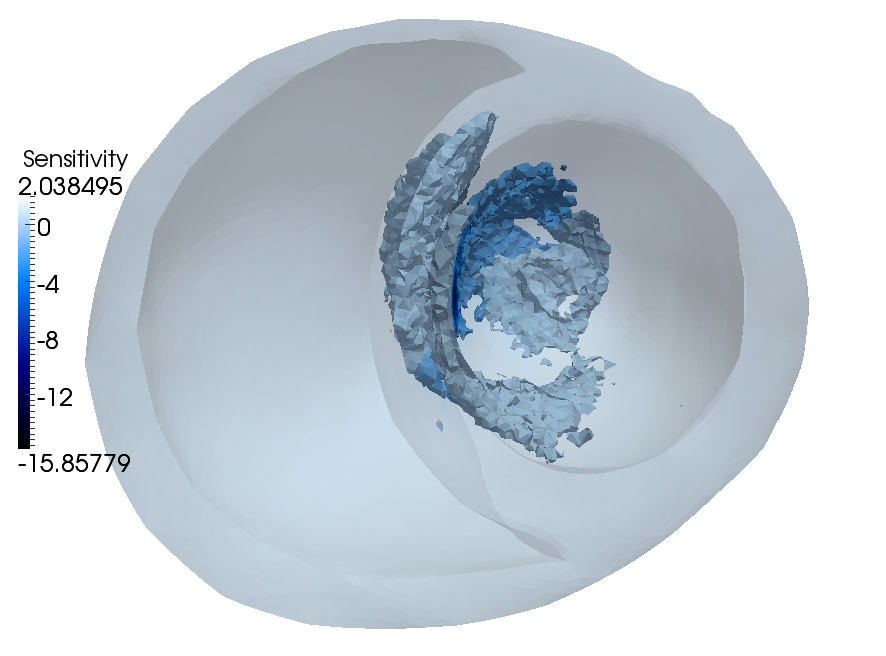
\includegraphics[width=0.49\textwidth]{png/g_el_plusx.png}
  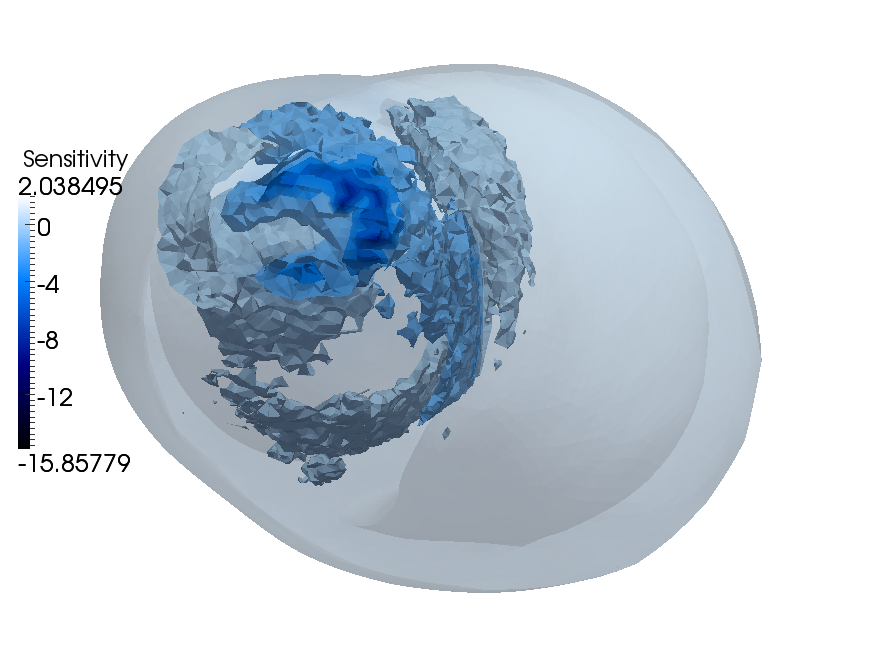
\includegraphics[width=0.49\textwidth]{png/g_el_minusx.png}
  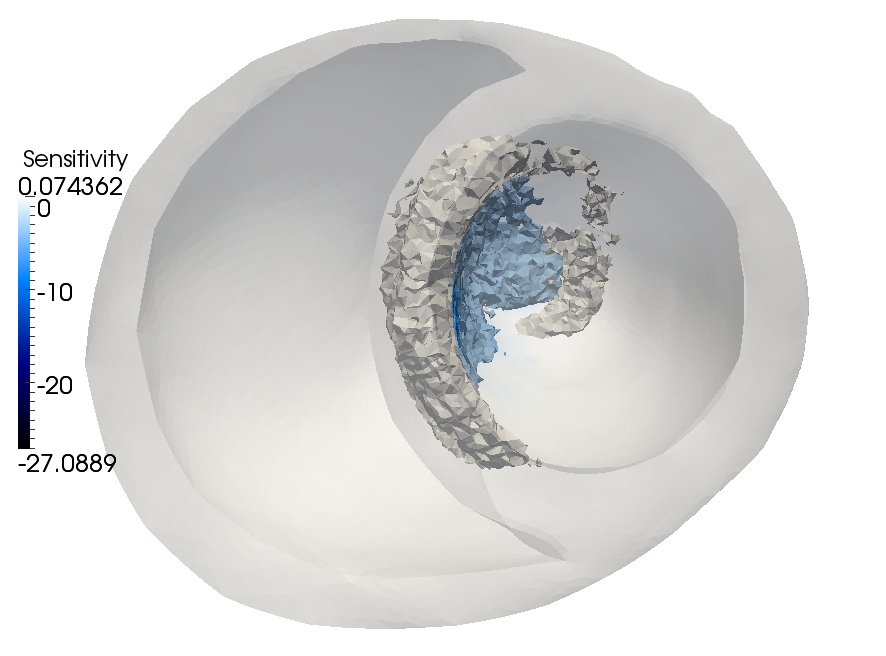
\includegraphics[width=0.49\textwidth]{png/g_et_plusx.png}
  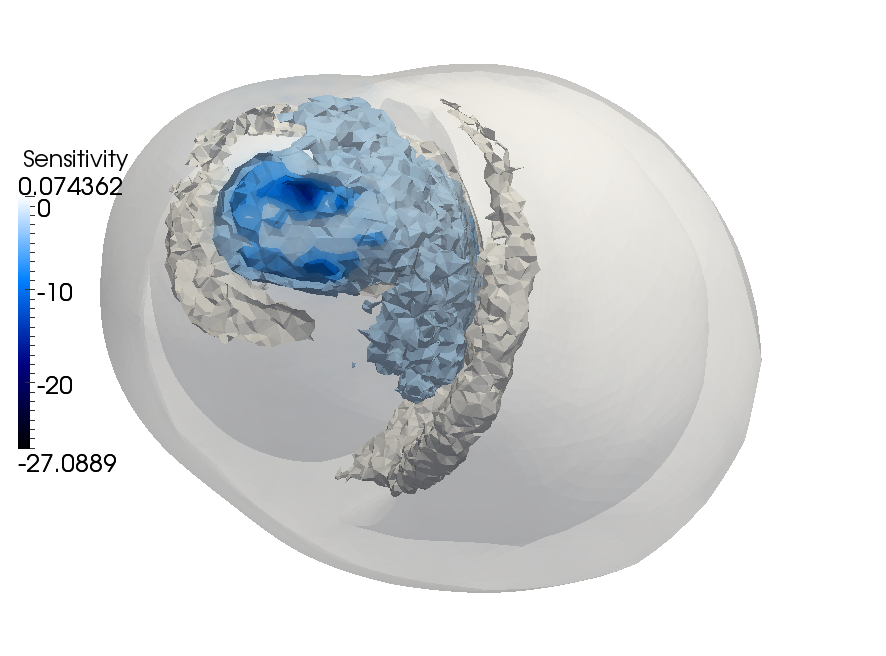
\includegraphics[width=0.49\textwidth]{png/g_et_minusx.png}
  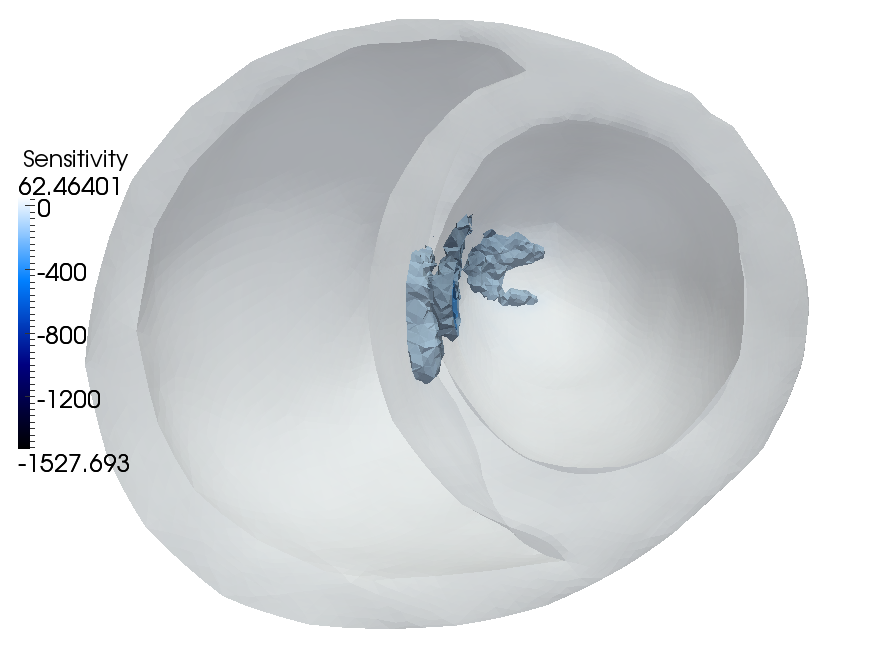
\includegraphics[width=0.49\textwidth]{png/g_il_plusx.png}
  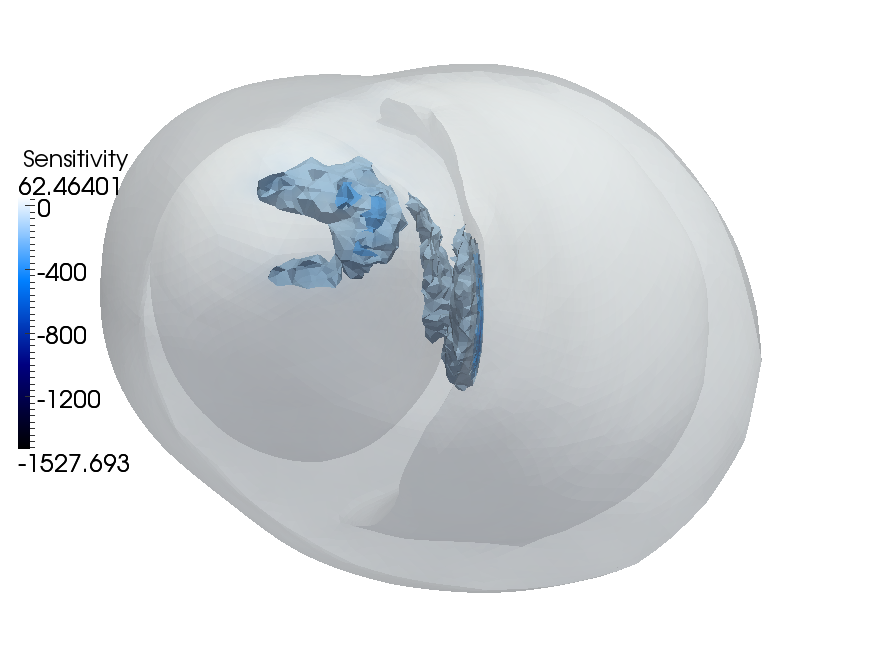
\includegraphics[width=0.49\textwidth]{png/g_il_minusx.png}
  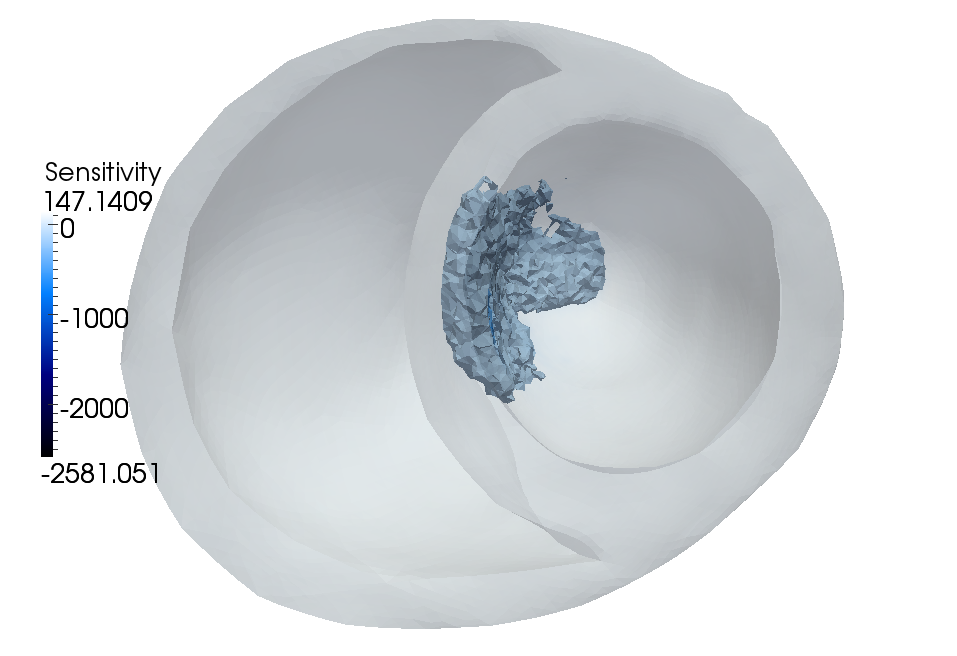
\includegraphics[width=0.49\textwidth]{png/g_it_plusx.png}
  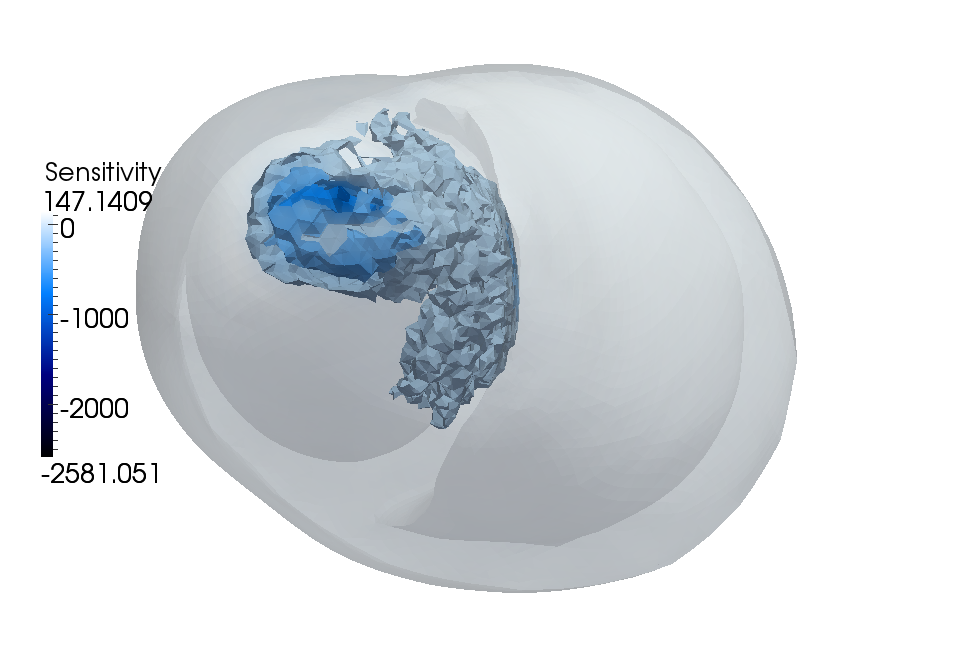
\includegraphics[width=0.49\textwidth]{png/g_it_minusx.png}

\caption{Adjoint sensitivity maps of functional described in
  Figure~\ref{fig:user-code-adjoint} with respect to (from top to
  bottom) $g_{el}$, $g_{et}$, $g_{il}$, $g_{it}$. For each, the right
  figure shows camera view from positive x-axis on the right (looking
  down at the ventricles), and the left figure shows camera view from
  negative x-axis (looking up at the ventricles). Large values (either
  positive or negative) indicate high sensitivities. Note the
  differences in scaling (the numbers on the colorbar). }
\label{fig:sensitivity-maps}
\end{figure}


\bibliographystyle{siam} \bibliography{bibliography}

\end{document}
